\documentclass[a4paper,14pt]{memoir}
\usepackage{tipa}
\usepackage{tgschola}

\usepackage{graphicx}
\graphicspath{
	{pics/}
}

\usepackage{xcolor}
\usepackage{pagecolor}
\usepackage{afterpage}

\usepackage{hyperref}

\usepackage{tikz}
\usetikzlibrary{shapes.geometric}

\setlength{\parskip}{\baselineskip}%
\setlength{\parindent}{0pt}%

\newcommand{\mtr}[1]{\textbf{#1}}
\newcommand{\bigmtr}[1]{\begin{center}\large \mtr{#1} \end{center}}
\newcommand{\sadhaka}{sādhaka}
\newcommand{\mudra}{mudrā}
\newcommand{\asana}{āsana}
\newcommand{\sadhana}{sādhanā}
\newcommand{\Vamacara}{Vāmācāra}
\newcommand{\Kali}{Kālī}
\newcommand{\Mahavidya}{Mahāvidyā}
\newcommand{\Tara}{Tārā}
\newcommand{\TripuraSundari}{Tripura Sundarī}
\newcommand{\Lalita}{Lalitā}
\newcommand{\Shodashi}{Śoḍashī}
\newcommand{\Bhuvaneshvari}{Bhuvaneśvarī}
\newcommand{\Chinnamasta}{Chinnamastā}
\newcommand{\Bhairavi}{Bhairavī}
\newcommand{\Dhumavati}{Dhūmāvatī}
\newcommand{\Bagalamukhi}{Bagalamukhī}
\newcommand{\Matangi}{Matāngī}
\newcommand{\Kamala}{Kamalā}
\newcommand{\prana}{prāṇa}
\newcommand{\pranic}{prāṇic}
\newcommand{\apana}{apāna}
\newcommand{\apanic}{apānic}
\newcommand{\kundalini}{Kuṇḍalinī}
\newcommand{\shakta}{Śakta}
\newcommand{\shakti}{Śakti}
\newcommand{\Shiva}{Śiva}
\newcommand{\muladhara}{Mūlādhāra}
\newcommand{\svadhisthana}{Svādhiṣṭhāna}
\newcommand{\manipura}{Maṇipūra}
\newcommand{\yoni}{yoni}

\newcommand{\cmmnt}[1]{\textcolor{red}{#1}}


\newcommand{\colorcirco}[2]{\tikz\draw[#1,fill=#2] (0,0) circle (1ex);}
\newcommand{\colorcirc}[1]{\colorcirco{#1}{#1}}

\begin{document}

\title{Erotic Esoterics}
\author{cancrizans canon}

\makeatletter
\begin{titlingpage}
\pagecolor{black}
\color{white}

\centering
{\bfseries\fontsize{50}{60}\selectfont \@title}\\[\baselineskip]
{\scshape practical tantrik manual to occult sexuality}\\[\baselineskip]

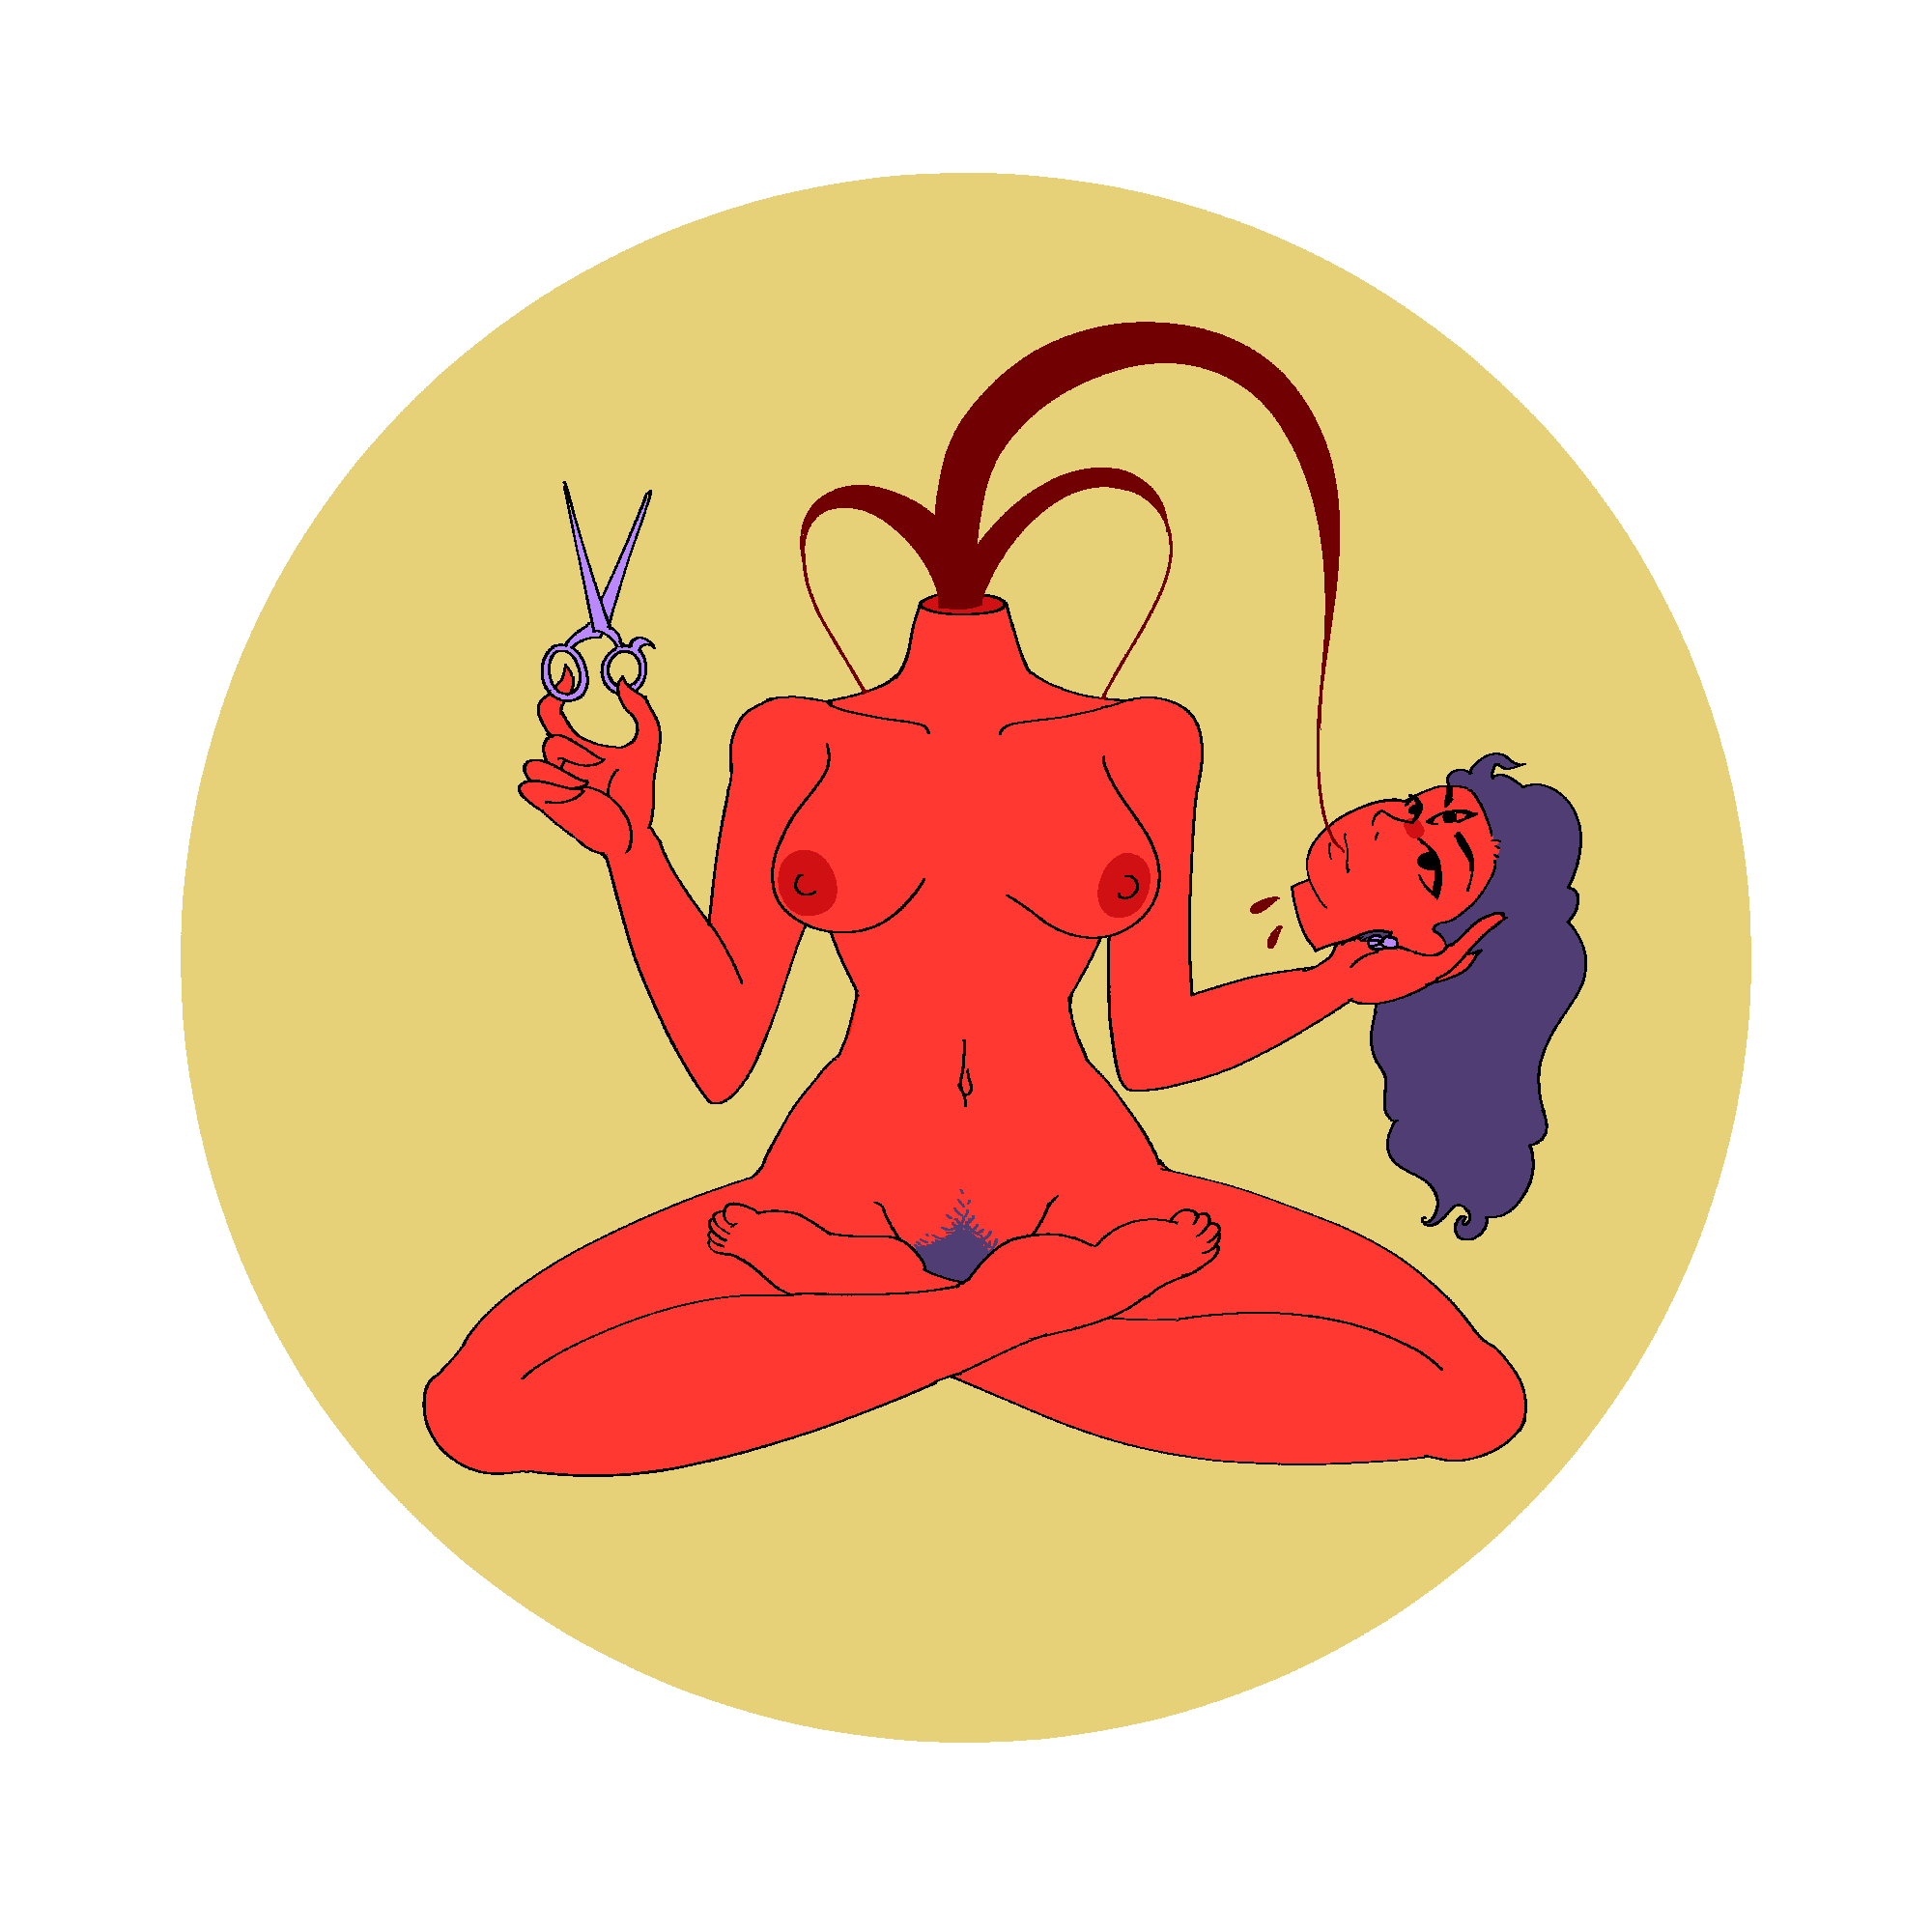
\includegraphics[width=6in]{chinna.png}

{\large\scshape \@author}
\afterpage{\nopagecolor}
\end{titlingpage}

\begin{titlingpage}
\centering
{\Huge\bfseries \@title}\\[\baselineskip]
{\scshape practical tantrik manual to occult sexuality}\\[\baselineskip]

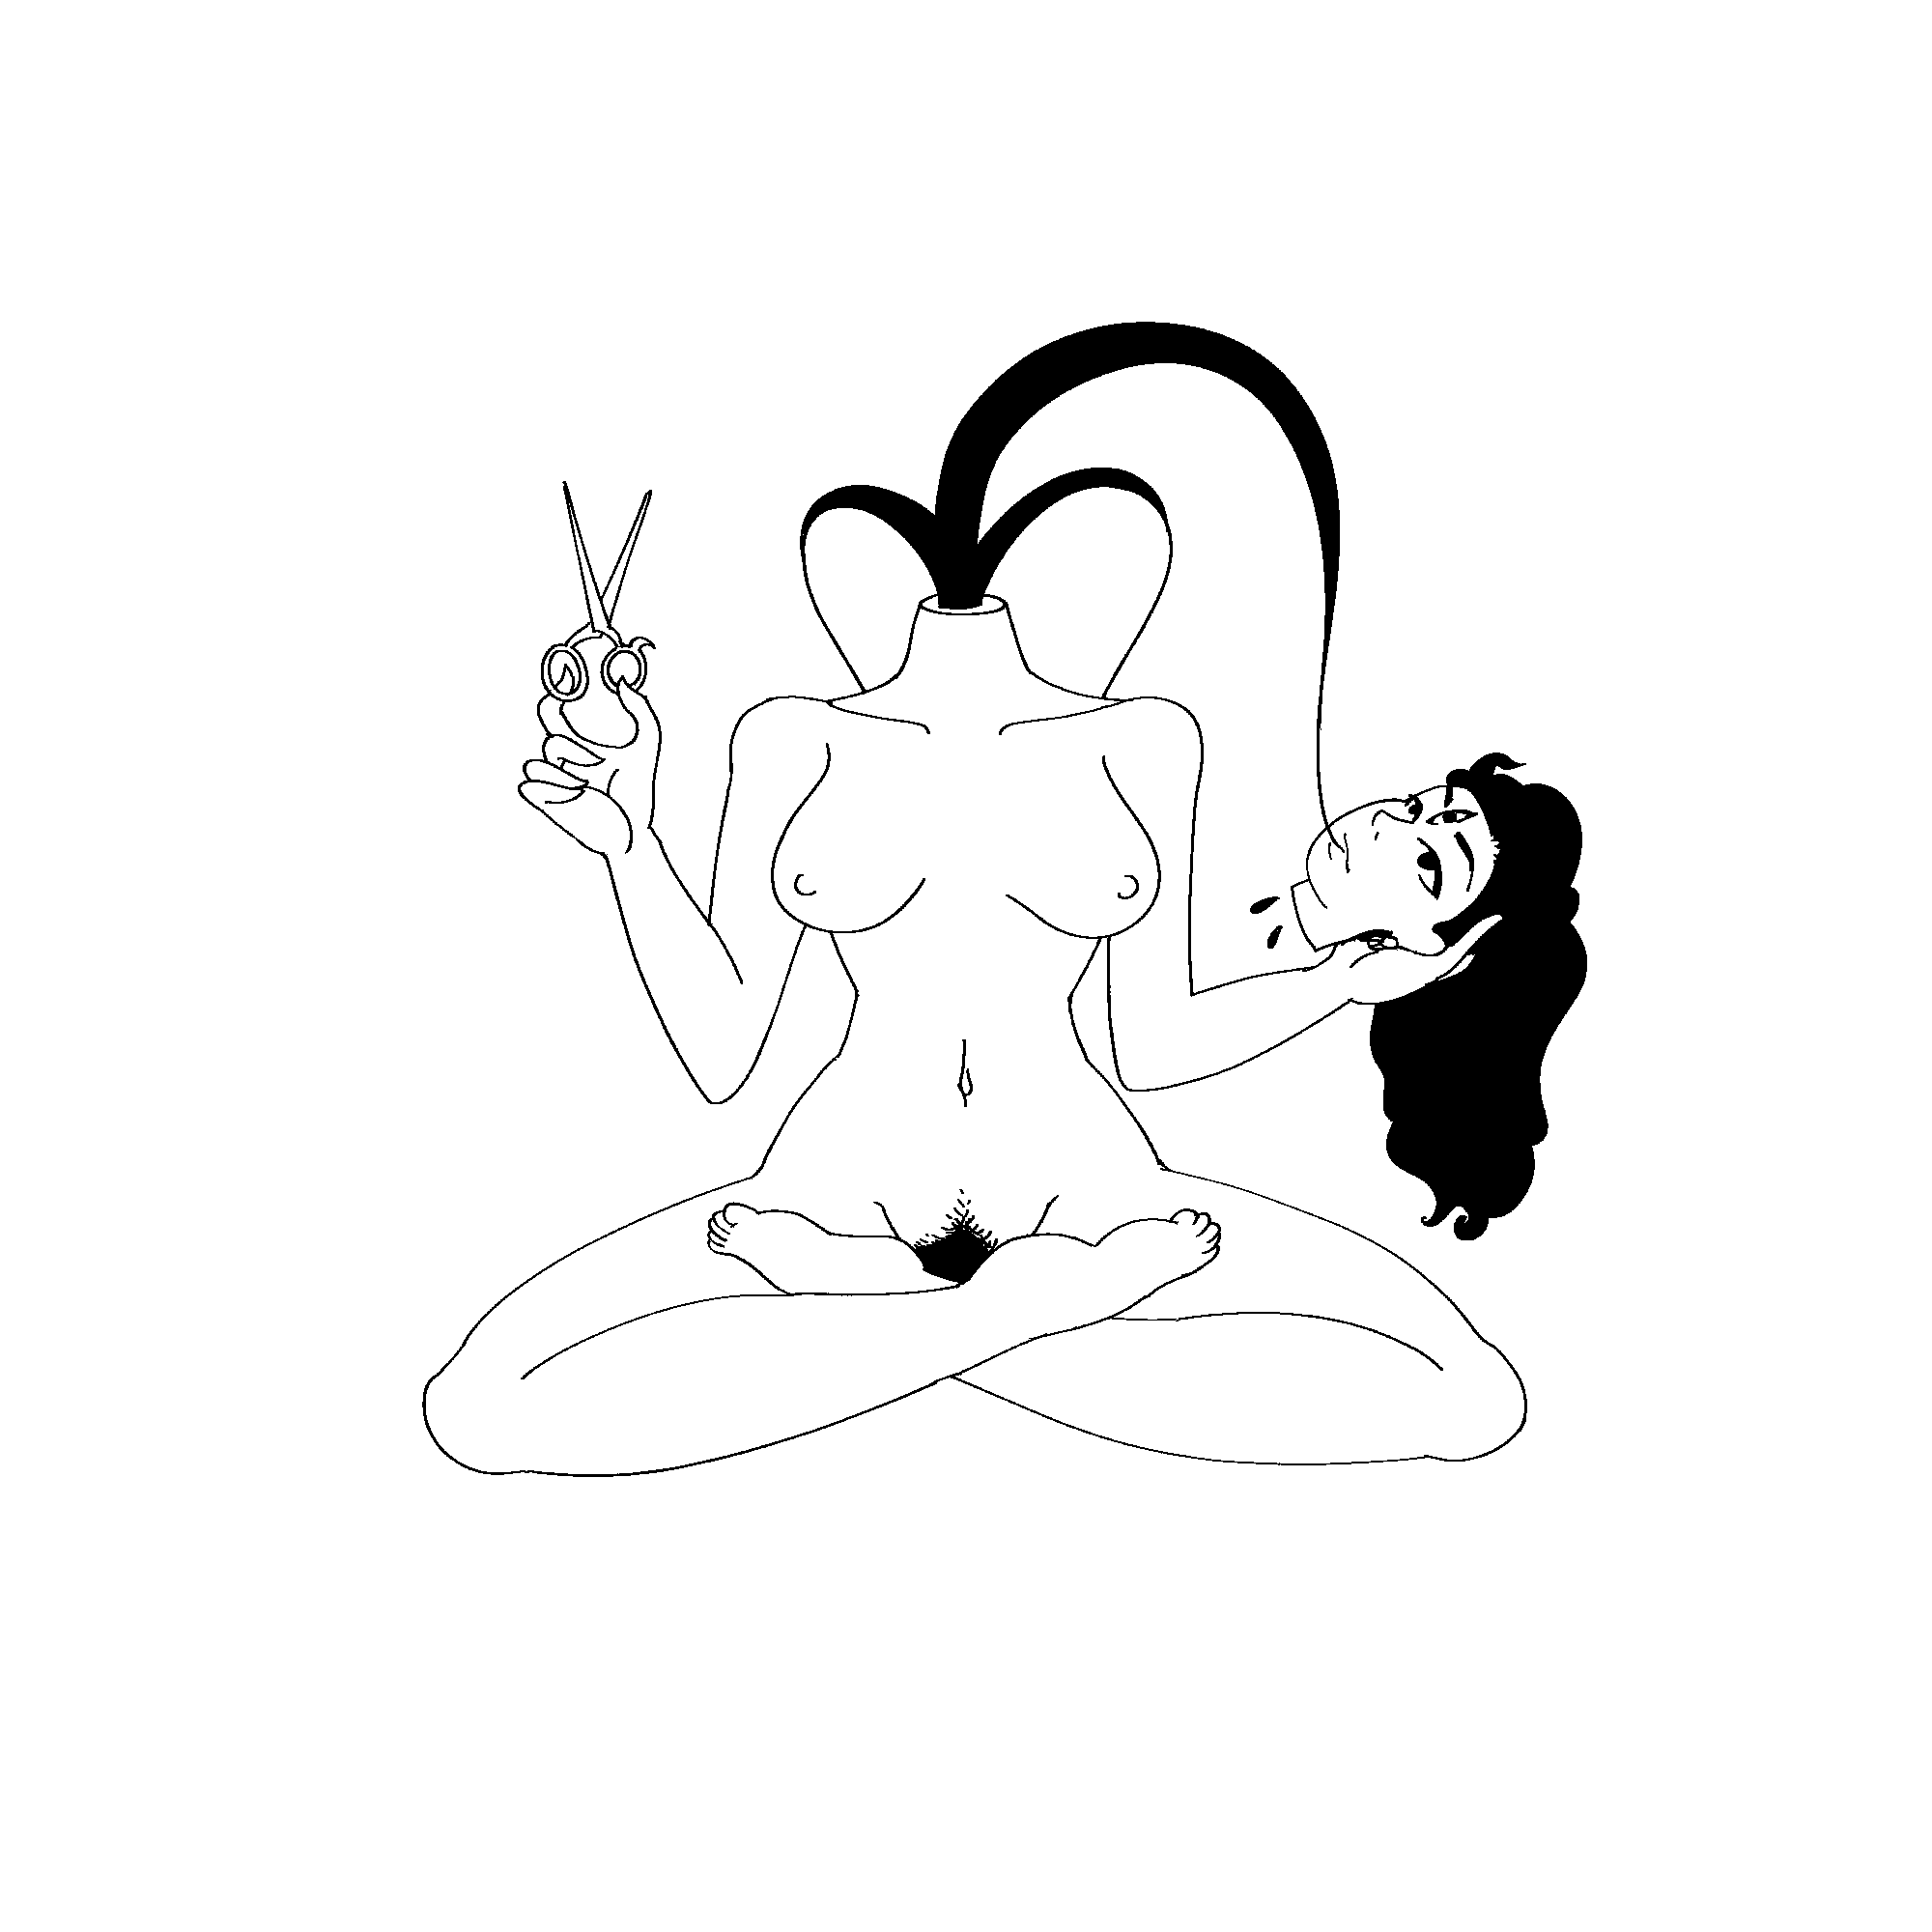
\includegraphics[width=6in]{chinna_bw.png}

{\large\scshape \@author}
\end{titlingpage}
\makeatother

\section{Foreword}

Few human experiences lead to divinity as brilliantly and spectacularly as fucking.

Though it would be an understatement to say sex is a complicated ordeal. As a source for any kind of transcendent insight, or spiritual growth, or a magical dimension, it's quite ill-suited on the face of it. It's unfair, unequal, distracting, feverish, mercurial. It's filthy, basal, hydraulic. It feeds jealousy, bitterness, shame, and all sorts of heartburns and stomach acidities. Demands utmost care, guidance and wisdom to not devolve into its supposed natural conclusion of violence. In fact, in the picture we hold of it in our modern lens, sexual desire is a true calling to the violence and stupidity of the animal nature within man, one which must be held at bay, reasoned with, tricked into civilisation. Tamed, and trained, as the wolf is funneled into the mould of the domesticated dog.

A more rebellious current of sexual liberation wants to unlock the cage and allow such beast to roam free, drinking full from the rivers of pleasure. While we have to thank this spirit for the freedoms we enjoy to explore our intimacies unburdened by moral norms, it is underlied by an unspoken germ of disorienting optimism. The young person diving into the highs and lows of sex, exhilarated by the understanding that as long as love is involved, no sex is wrong, as in immoral, might be persuaded, or might persuade themselves, that sex can do \emph{no wrong}, that it is ultimately harmless, meaningless, consequence-free. That the spring of sexuality is a never-ending source of a pleasure that is disjoint from all other aspects and hardships of life - a pocket universe where all troubles are forgotten and one may sink, or play out as many absurd colourful scenarios as the mind can imagine, and then return to waking life unscathed, unaffected, bringing neither boons nor battle wounds. As if it never happened.

I'll spare you the obvious conclusion: there must be a third way, one where sex is neither suppressed, nor trivialized, but allowed to blossom into new forms, transmuted into more than the sum of its parts, and powerful beyond imagination. In this little manual, or call it a notebook, I try to describe to you how to walk this narrow path, and hopefully the information I've collected will be of any use to you.

This booklet describes a \sadhana{}, which means a spiritual path including many practices, which you are free to undertake in part or whole. None of this you should take on authority nor faith -- rather, you should experience and evaluate these insights by yourself on your own skin, and incorporate them only if they end up being accurate and useful. For the purpose of enforcing this, I won't be talking much about myself and my background, nor will I pontificate about metaphysics and philosophy and all such very intellectual means by which people are led to waste time debating (when they could be making love), and I'll only explain what I need to make my point or explain a certain procedure. We'll skip over the entire question of guruhood and transmission, even though it's very important to tantra, and you are free to call yourself a \sadhaka{} or anything else. You have genitals, and as we will see genitals are an antenna for otherworldly revelation - you already have guidance, and all we need is to learn how to listen.

Speaking of, this path is open to you no matter what your biological sex, gender, or sexual orientation are. Some esoteric aspects of sexuality are universal, other do depend on these variables, but I'll try to cover all cases I can where possible. For convenience, I'll be talking about ``men'' when referring to people with a penis, and ``women'' for people with a vulva and a vagina, but this simply means that what I have to say is focused on the specific of the genitals, and it's not a statement about who has the right to identify as what. In tantra, the body is the primary magical tool and spiritual dimension. If you're, say, a pre-op trans woman, you'll probably be at least mildly annoyed to read me gushing about the cosmic power and trascendent potential of that ugly thing between your legs that you could easily do without, but I ask to you to meet me halfway and give it a chance for its mysteries to blossom. A person with mastery of all sexes and genders is an awe-inspiring force, and the first step on that path is communion with your body as it is now.

\tableofcontents

\chapter{Spiritual Sexuality}

\section{Basics of \shakta{} and \kundalini{} tantra}

\cmmnt{more}

For our purposes, we focus more on the lower section of the subtle body, the endpoint connected to the immanent and feminine polarity. Keep in mind that \kundalini{} rises - this significant inner motion is symbolic of a distillation or transmutation process, wherein we begin from the lowest depth of the underworld and blossom upwards into the heavens, transforming in a process. This journey begins from the gross plane, the material realm. Our journey begins in filth. This is why tantra reads the body in the order from bottom to top.

There are three principal classical cakras in this lower half. Cakras can be described as psychosomatic loci, or psychically significant nodes, structural in the mind's map of the body, or the body's connection to the mind (primarily through the nervous system). One picture which I personally find very useful especially but not only for the lower cakras is to imagine them as sphincters or valves. A "blockage" is maybe more eloquently described as a clenching or tension which impedes a subtle flow. In an unaware state, this tension is applied as a form of habit due to fears and other negative emotions, and so in the practice of tantrik yoga one of the goals is to specifically relax those tensions, establish a practice of opening these ``valves'', and allowing free flow of currents.

The three lowest classical cakras, from the bottom, are:

\subsection{\muladhara{}}

\textbf{\muladhara{}} is rock bottom, the root of the world. This psychic locus is so real, so immanent, so alive and true, that it actually lies physically outside of the body, almost out of the reach of the mind. It is located in the empty space slightly below the perineum, but the better way to understand it is that \muladhara{} is the bridge connecting the person to the rest of physical existence. The root is our literal, material, every day adult life. It's a window into the world, bursting with life and death, suchness and solidness. It's the ground beneath your feet.

Within the body, \muladhara{} is connected to the coccyx, the coccygeal plexus, and most importantly the \textbf{pelvic floor muscles}. The subtler notion of the root of the world is reflected in the pelvic floor's function as support for the weight of internal organs. In fact, the architectural analogy for the body in yoga makes \muladhara{} a literal foundation, in its element when weight is confidently discharged through it.

It is also associated with all transits and exchanges of material from the living body to the external world, in particular urination and defecation. Death and putrefaction are the ultimate realisation of the spirit of \muladhara{}, the gates of the root opening and the microcosm of the person dissolving its life into the larger environment. Life is not lost, just passed on - \muladhara{} is specifically that exit.

The element of \muladhara{} is the \textbf{Earth}, obviously, and its seed mantra is \textbf{laṃ}.

\subsection{\svadhisthana{}}

\textbf{\svadhisthana{}} 

\subsection{\manipura}

\textbf{\manipura}{}

\section{Subtle Sexual Anatomy}

Our previous understanding of sexuality as society taught it to us was probably overall very straightforward: we imagine that, say, a man walks in the direction of a certain sexual pleasure, acting so as to maximise it. When the pinnacle of such pleasure, the destination of the longing, is reached, we have a little celebration with a final burst of satisfaction and the genetic payload is delivered.

This cartoonish picture is structurally flawed and is one of the major ingredients for the disastrous levels of confusion over the workings of the penised individual. I'll try and sketch out an improvement upon it. We don't need to elucidate all details on the metaphysics of sex, nor all of the actual relevant medical fields - we just need the bare minimum of observations to be able to operate this strange machine properly.

``Sex drive'' is really composed of two differently-directed aspects, seeking two distinct goals. There is a life-seeking libido, the \textbf{\pranic{} drive}, and a death-seeking libido, the \textbf{\apanic{} drive}. The \apanic{} drive strives for orgasm and ejaculation, which are dissolution and expulsion of life-giving fluid. The \apanic{} libido wants you to come undone and disperse your life energy into the rest of the universe - it's self destructive, ravenous, and feverish. It follows closely the dopamine-rich intense pleasure of sexual stimulation and the approach and reaching of orgasm, which has a restless, intoxicating and addictive quality. Instead, the \pranic{} drive is much calmer, and its purpose is to \emph{preserve} internal life. It is quieter, sharper, and we associate it with seeking much subtler pleasant feelings of satisfaction, ecstasy, etc. It wants the life-energy produced in sex to be redirected inwards and upwards to be distillated into a more refined form. The \pranic{} drive exists because if we were only moved by the \apanic{} flow, we would just seek ejaculation as soon as possible, and as much basal pleasure as the body will allow, and would have no interest in actual sex between humans, an act which is wholly inefficient for that purpose.



\section{Transmutation}

\section{Divine Gender}

\section{Power and Morality}

\section{Erotic Devis}

The \textbf{Ten \Mahavidya{}s} (Great Wisdoms) are a group of tantrik goddesses. They are tantrik in the sense that their significance is mainly esoteric and their \sadhana{}s (associated practices) are occult. All of them are specified aspects of the primary feminine principle of \shakti{}; the purpose of these deities is to focus on particular features of a vast and potentially too abstract concept to isolate and work on subcomponents of it. Some of them are darker / fierce expression of that energy, and some of them are more positive (yet still mysteric). Here I want to talk about specifically the sexual interpretation of the ten \Mahavidya{}s, as each of them is associated with a specific esoteric process associated with sexuality.

In the most common classical order (the order holds no particular meaning):

\begin{itemize}
	\item \colorcirc{black} \textbf{\Kali} - she is a ``root'' \Mahavidya{} and incorporates the other nine as sub-aspects.
	\item \colorcirc{blue} \textbf{\Tara}\footnote{The hindu \Mahavidya{} \Tara{} is continuously connected to the Buddhist \Tara{}, but it's important to mantain the distinction due to the strong differences in character and iconography that have accumulated over time. Worship of the \Mahavidya{} \Tara{} is overall much rarer, and even within a large degree of variation she is a significantly darker figure than the Buddhist \Tara{}.} is the fearsome Mother. She is pot-bellied, but for us she might as well be heavily pregnant, dancing in the cremation ground. She is the power of constant renewal of life throught death inherent in the \textbf{reproductive aspect} of sex, and the intoxicating and potentially dangerous figure of the protective, motherly/fatherly partner.
	\item \colorcirc{pink} \textbf{\TripuraSundari}, aka \textbf{\Lalita} or \textbf{\Shodashi}, is the \textbf{Hierogamy}, or sacred intercourse, of the masculine and feminine principles. She is central to the Śrī kula family of \shakta{} tantra, and she is associated with the Śrīyantra, the mechanism of the subtle coitus between \Shiva{} and \shakti{}.
	\item \colorcirc{orange} \textbf{\Bhuvaneshvari} is the \textbf{Cosmos as a Woman}. She is the humbling vastness of the physical universe and all natural phenomena. Science is intercourse between the abstraction of the intellect and the supple truth of \Bhuvaneshvari{}.
	\item \colorcirc{violet} \textbf{\Bhairavi} is a terrible goddess of annihilation, the silence after the end of the world. She is \textbf{Death in Orgasm}.
	\item \colorcirc{red} \textbf{\Chinnamasta}\footnote{The origin of \Chinnamasta{} traces back to the Buddhist headless vajrayogini Chinnamundā. The figures share many features on the surface, but are significantly different in the metaphysical suggestions of the violent act of self-decapitation.} the self-beheaded is \textbf{Sexual Transmutation} through coitus reservatus. She sublimates libido into a purified form of spiritual nourishment for herself and others, shedding the bindings of her ego, and becoming more than the sum of her components. \Chinnamasta{} is the primary sexual tantrik Devi.
	\item \colorcirc{gray} \textbf{\Dhumavati} is an old crone. She can point to \textbf{Beauty in Ugliness}, and mediates the sophistication of desire and arousal with the onset of the wisdom of age.
	\item \colorcirc{yellow} \textbf{\Bagalamukhi} is the \textbf{Sex Magician} - she deliberately uses the tools at her disposal to manipulate her surroundings to her benefit.
	\item \colorcirc{green} \textbf{\Matangi} is the outcast practitioner of all forbidden arts. She is \textbf{Perversion}, a violator of sexual taboo. \Matangi{} dances with shame, and appreciates the intricacies and unique boons that come with immoral sexuality.
	\item \colorcirco{gray}{white}  \textbf{\Kamala} is the Lotus, \textbf{Enlightenment}. She is the innermost mystery and the eternally-sought destination of the dharmic spiritual path. In our tantrik approach, we will attempt to know \Kamala{} by heterodox means.
\end{itemize}

\subsection{\Chinnamasta}

\cmmnt{Re-edit section}

Chhinnamasta is the self-decapitated figure. Her story \& iconography has many variants and she even has a buddhist equivalent as a vajrayogini. In one story Parvati bathes in a river and becomes sexually aroused, and her skin turns black (symbolic of fierceness). Meanwhile her two attendants are hungry and beg her for food. Parvati severs her own head with her fingernails and the three jets of blood nourish both attendants and the devi's own living head.

This shocking imagery is pregnant with symbolics. Chhinnamasta is passionate, but not overwhelmed by passion but rather exerts control and transformative redirection of passion. She is the tantrik goddess of sexual transmutation, or any sublimation of passion for that matter, and her abode is the burning fire of the solar disk of manipura, in the coeliac aka solar plexus. Passion, is, quite literally, beneath her, and she represents the refined form of controlled passion, forged by fire. Chhinnamasta is a paradox - sacrificing her head, her ego, she makes herself into more, and is able to provide spiritual sustenance for both others and herself to an extent which she couldn't with her head screwed on

The three spurts represent the subtle channels of ida, pingala and sushumna, and her head and two attendants the three gunas which the tantrika is called to cultivate.

1
[10:09]
The sexual position with the woman on top is relevant, but you have to understand it in context
[10:12]
1) this position is "forbidden", unusual, and inverts the typical hierarchy. It is inherently immoral (in the literal sense of against morae). This triumph of woman over man, Kali stepping on Shiva, or in subtle terms of the gross body and immanence dominating over the mind and transcendence, is inherently "not by the book" and tantrik/occult.

3
[10:17]
2) this is, as far as penetrative sex goes, and at least in the context of medieval india, the best position for sexual control, to effect transmutation of desire into creative or spiritually beneficial drives. Symbolically semen not spilled rises up from the underworld into higher sections of the person, purifying as it rises. This is kundalini's violent and devastating ascent, and Chhinnamasta's violent and sudden act mirrors that

cancrizans — 22/12/2022 10:29
In Shakta philosophy we always need to keep a layer of translation with regards to divine gender, and its relationship to earthly gender. Otherwise things don't make sense. The masculine principle (Shiva) is abstract, detached, logical, dispassionate, moral, disciplined, static and dead / inorganic. The feminine (Shakti) is the physical world, the body, the passions, she is impulsive, violent, alive, and impermanent. These are more or less just categories defined as is, then metaphysics worries about what is real where and how and dualities and non-dualities. Interesting but not right now. It is true that everyone no matter the gender has a body and a mind, and one is called to work with these principles to become a balanced and well shape person. Chhinamasta's form of the dark divine feminine is one of specifically transformative power. She couldn't be a male god because the divine masculine does not have that potential to change nor the vantage of using physicality to effect it. And this is the esoteric meaning behind Chhinamasta being not just any woman, but very feminine: depicted as youthful and attractive. Almost a fertility goddess, yet the intention behind that sexual act is completely inverted

6
[10:30]
Her sadhana is tough, very difficult to find information on, and of course the practice is only left-handed.

\chapter{Practice}

\section{Basic Meditation}

\cmmnt{Edit this}

Super basic meditation 101 for absolute noobs

Meditation is first of all an exercise in presence. Presence / mindfulness is simply full and direct awareness of your immediate surroundings and inner state. No imagination, paranoia, memory, vision, hypotheticals... just the thing as it is, focus on your literal immanent present. Meditation's purpose is not to reach this "state" but to cultivate it as a skill or habit - presence trained in meditation lingers on for the rest of daily life. This is the goal.

It's a simple exercise you do every day to keep your mind-body into that good shape. To do it however we do need to set up the body in a configuration that is conducive to that good work, otherwise it's going to be counterproductive.
[19:07]
Legs and spine

The ideal asana (pose) for meditation is probably the full lotus or half lotus, but unless you're already a yoga freak and/or started out pretty flexible, you're not gonna be able to jump into that without injuring yourself. On the other side of the spectrum, sitting simply cross-legged with both feet under the knees (sukhasana) is gonna take a toll on the quality of your meditation, and if you're not flexible enough for the more stable asanas, I would recommend meditating sitting on a chair, something high enough that your knees are at 90°. Imho it's better than cross-legged.

The reason why we worry about the pose here is that we do need to think about the body in an architectural sense. It's a building that must discharge its weight loads into the support (floor or chair). It must do so in a way that doesn't leave any parts oscillating or "hanging" under stresses, because to hold that body part in place we'll have to use our muscles, and it will wobble, and that's gonna be hell for our focus! Human beings have MASSIVE heavy heads. Megamind. They are built like spoon. So we're going to need to unload the weight of the head through the spine, down straight all the way through the spine until we reach the coccyx / perineum. This is muladhara, the root of the world, the truth of the ground beneath your feet. Then, if we are in lotus, the weight unloads from there through the legs and into the ground, since the legs form a stable (non-wobbling) base to discharge all that weight. Someone in that position is truly a building, and their body is a tower connecting heaven and earth. Solidity => less distractions.

As beginners we can try and do our best here, make sure your spine is straight, no slouching, no instagram thot arching, just straight.
[19:11]
Eyes
Many different opinions here. You have the option of closed eyes meditation, or you can keep them open, ideally with your gaze a bit under straight ahead, like 10° downwards. Just make sure not to doze off. Both have pros and cons. Closed eyes can lead to too much visualizing and distraction, and might not be ideal for a daily base practice. Imho it's better to leave closed eyes for more specific work. Open eyes keep you grounded into the suchness of the present moment in which you are actually in a room meditating.
[19:16]
Hands
Hand pose is called a mudra. Most definitely go with dhyana mudra, meaning the hands are open palms up and one cupping the other, just relaxed and laying in your lap. Let the thumbs touch. Thumbs can be used as a monitor during meditation. If they separate, you are dozing off and getting too relaxed, if you feel an uncomfortable pressure, you are too stressed. Make sure the hands are just "laying there" and that you're not making any effort with your muscles to prop them up in place. Your arms should basically be as good as dead.

Since we're there, your shoulders should be relaxed and hanging low. You can take a deep breath and let them drop on the exhale, and you'll see how much in your daily life they're all clenched up and you never even notice
[19:17]
Mouth
In basic meditation, you will be breathing through the nose, never through the mouth. Keep the mouth slightly ajar. Place your tongue gently but firmly pressed on the alveolar ridge (just say "nnnn....", that's your tongue pose). In this posture, if you do it well, you will not salivate anymore. Not having to gulp helps a lot.
[19:21]
Breath
Obviously, deep slow careful breaths in and out through the nose. The good spine posture will really make a difference in the ease of deep breathing - slouching can make you short breathed fast. Now you're gonna want to do something that sounds easy but really isn't. When you inhale, you want to blow up first the lower parts of your lungs, raising the diaphragm, and then filling up to expand the  chest. As you exhale you squeeze the lungs starting from above, deflating the chest but squeezing the air in the abdomen, then finally exhaling that last bit slightly forcefully. Don't overdo it, just a bit of this squeezing from above.

cancrizans — 20/12/2022 19:31
Ok then how the hell do I actually do it?
Prepare a room where you won't be disturbed for at the very least 20 mins. I recommend doing this in the early morning, but you do you. You wanna avoid moments where you're exhausted and about to fall asleep. Wear comfortable clothes, be naked if it works for you. Plop your ass on the floor or chair (or a pillow - pillow under the spine and legs on the floor, the height difference helps make certain asanas more accessible and makes your more stable). 

Then slowly go through the things I explained to you before, this is your checklist and following it is your task. I check my mouth position. I check my hands. Maybe I'll focus on how my toes feel from the inside. Then I check my spine is straight. Then my shoulders. Then idk the mouth again. You just cycle through, slowing your breath, lowering your shoulders. Becoming more and more involved with the mechanics and details of being here right now.

When a thought comes and tries to whisk you away, you don't fight it. You're not a fighter and you don't judge right now. You just let it politely go. You're too busy with your list. You're too busy sitting here right now. 

This already is meditation and some great one at that if you can manage this for at least 10 minutes. Then you increase to 15 minutes at least, more if you want. Slowly day after day. It definitely is not a competition. It is the thing that is least a competition in the world. You can use an alarm clock if you like it or not if you're not the type; it's allowed.
[19:32]
As you can see the body is as much as involved as the mind. There is no boundary between them really, and it shows here. So beware of snake oil like people who claim they meditate in bed, or that after 65 minutes of meditation they started seeing ghosts and spirits. Not what we're doing. What we're doing is just sitting here, and practicing being really good at just sitting here, sharply awake. Nowhere else but here.

forgot to add something about earbuds and audio / music. If you can have silence, use the silence. If you live somewhere really noisy, then there's nothing wrong with wearing some earbuds and cranking up some ambient music or white noise. Don't bother with any guided meditations or anything with people talking. Listening to another person who isn't actually there talking is the exact opposite of what you're trying to do...

\section{Cleansing and Initiation}

It is not possible, or it is very difficult, to directly turn a regular sex life into a magical or spiritual one directly. The primary reason is the distracting and clouding effect of an undirected or undisciplined \apanic{} drive, anxieties, shames, and other bindings. These distractions embedded in your sexual habits can mask many important subtle sensation, or dull many revelations and insights. A spiritual practice where you don't feel the work happening is as good as dead.

Thankfully, it is possible, with patience, to first undo completely your previous habits. Sexuality does have the functionality to be ``reset'', though this has to be done correctly and carefully. You will have to make a commitment for a period of asceticism where you will ``flush out'' your whole current tangle, or at least create some distance from it, and accustom yourself to the subtler sensations that matter. But then, when the time is ripe, you will need to act intelligently to guide yourself to be reborn into a new sexual dimension; this is a delicate and difficult step and the danger is regressing into your old state. Remember: abstinence does not unmake a sexuality, it merely creates the opportunity for transformation.

You must think of this period as an initiation into these sexual mysteries. Do not see it as a permanent lifestyle - it works best when you understand it as transitional. It's a slow climb through a steep, dark path: eyes on the light on the summit. The duration of your first initiation should be no less than two months, and longer if you feel it necessary. At a later time, you may also refresh your involvement by performing a shorter initiation process again, like a 10-day ascetic period, but your first introduction will most definitely require a harder break. So err on the side of caution, and decide on a duration that you think will get you sufficiently close to being, on the level of instincts, essentially new to sex altogether. The initiate is ready when sex is as much of a discovery to them as when it was in puberty.

During your initiatory period, you will work to establish these habits, which I will explain in more detail below:

\begin{itemize}
	\item Do not masturbate or consume pornography in any form.
	\item Avoid entertaining sexual fantasies beyond the level of a passing thought
	\item Meditate and perform yoga every day
	\item Perform physical exercise every day
	\item Do everything in your power to sleep well
	\item Eat healthy
	\item Minimize intoxication
\end{itemize}

If this strict right-handed lifestyle sounds asphixiating, don't worry! It is meant to be, it's not permanent. It's a necessary sacrifice. It will teach you the skills of patience and will attune your spirit. It sharpens the blade of your Will.

\cmmnt{More}

\section{Yoga}

\cmmnt{More}

\subsection{Opening of the Seals}

This exercise helps develop relaxation, calmness and concentration during sex. It will improve sexual function, and it also has a strong potential to arouse \kundalini{}. It can be performed daily. Empty your bladder and assume a comfortable sitting \asana{} with a straight back.

\begin{itemize}
	\item Take several deep breaths, lower your shoulders, and take note of the sensations of the body. Take as much time as needed to be in presence. You can use a seven-limbed map to gain presence; the seven limbs are the head, the arms, the legs, the genitals and the coccyx. With each breath, observe the sensation of each limb until you feel at ease.
	\item \textbf{Unseal \muladhara{}:} Assume \apana{} \mudra{} with both hands. Take a deep breath, and during the inhale make sure to relax your anus and perineal muscles, almost like the breath continues into the pelvic floor and out of the body. During exhale, chant one long \textbf{laṃ} and try to maintain these muscles relaxed even though it's going to be harder than in the exhale. After the syllable is done, continue exhaling keeping relaxed. Repeat for 5 times.
	\item \textbf{Unseal \svadhisthana{}:} Assume \yoni{} \mudra{} and take a deep breath, and during the inhale relax and extend your PC muscle (visualise forcefully pushing out urine), imagining a warm energy flow from the sacral plexus in two lateral channels and into your penis or clitoris. For men, the flow passes through the testicles and rejoins into the penis, and for women, it splits much earlier, passes through the ovaries, alongside the channel of the vagina, and ends on the clitoris. In both cases, note how extending the muscle is like opening a dam for this flow which is more voluminous when this valve is unsealed. On the exhale, chant \textbf{vaṃ} and continue extending again against your instinct. Repeat 5 times.
	\item \textbf{Unseal \muladhara{}} again.
	\item \textbf{Unseal \svadhisthana{}} again, but now try to keep your anus relaxed as well in the meanwhile.
	\item \textbf{Unseal \manipura{}:} Assume \Kali{} \mudra{}. On inhale, push out your stomach as you inhale as much air as you can, and keep the entire pelvic area relaxed as just learned, almost like pushing your entire body out of your lower end. On exhale, suck in your stomach and lock the air below your sternum. Keep pushing out below and focus on the pressure of locked air trying to burst out upwards. Chant \textbf{raṃ}, then finally release the seal and allow air to escape. Maintain lower seals open. Repeat 5 times.
\end{itemize}



\end{document}